\section{Introduction}
% TODO: picture
\label{intro}

\begin{figure}[h]
    \vskip 0.2in
    \centering
    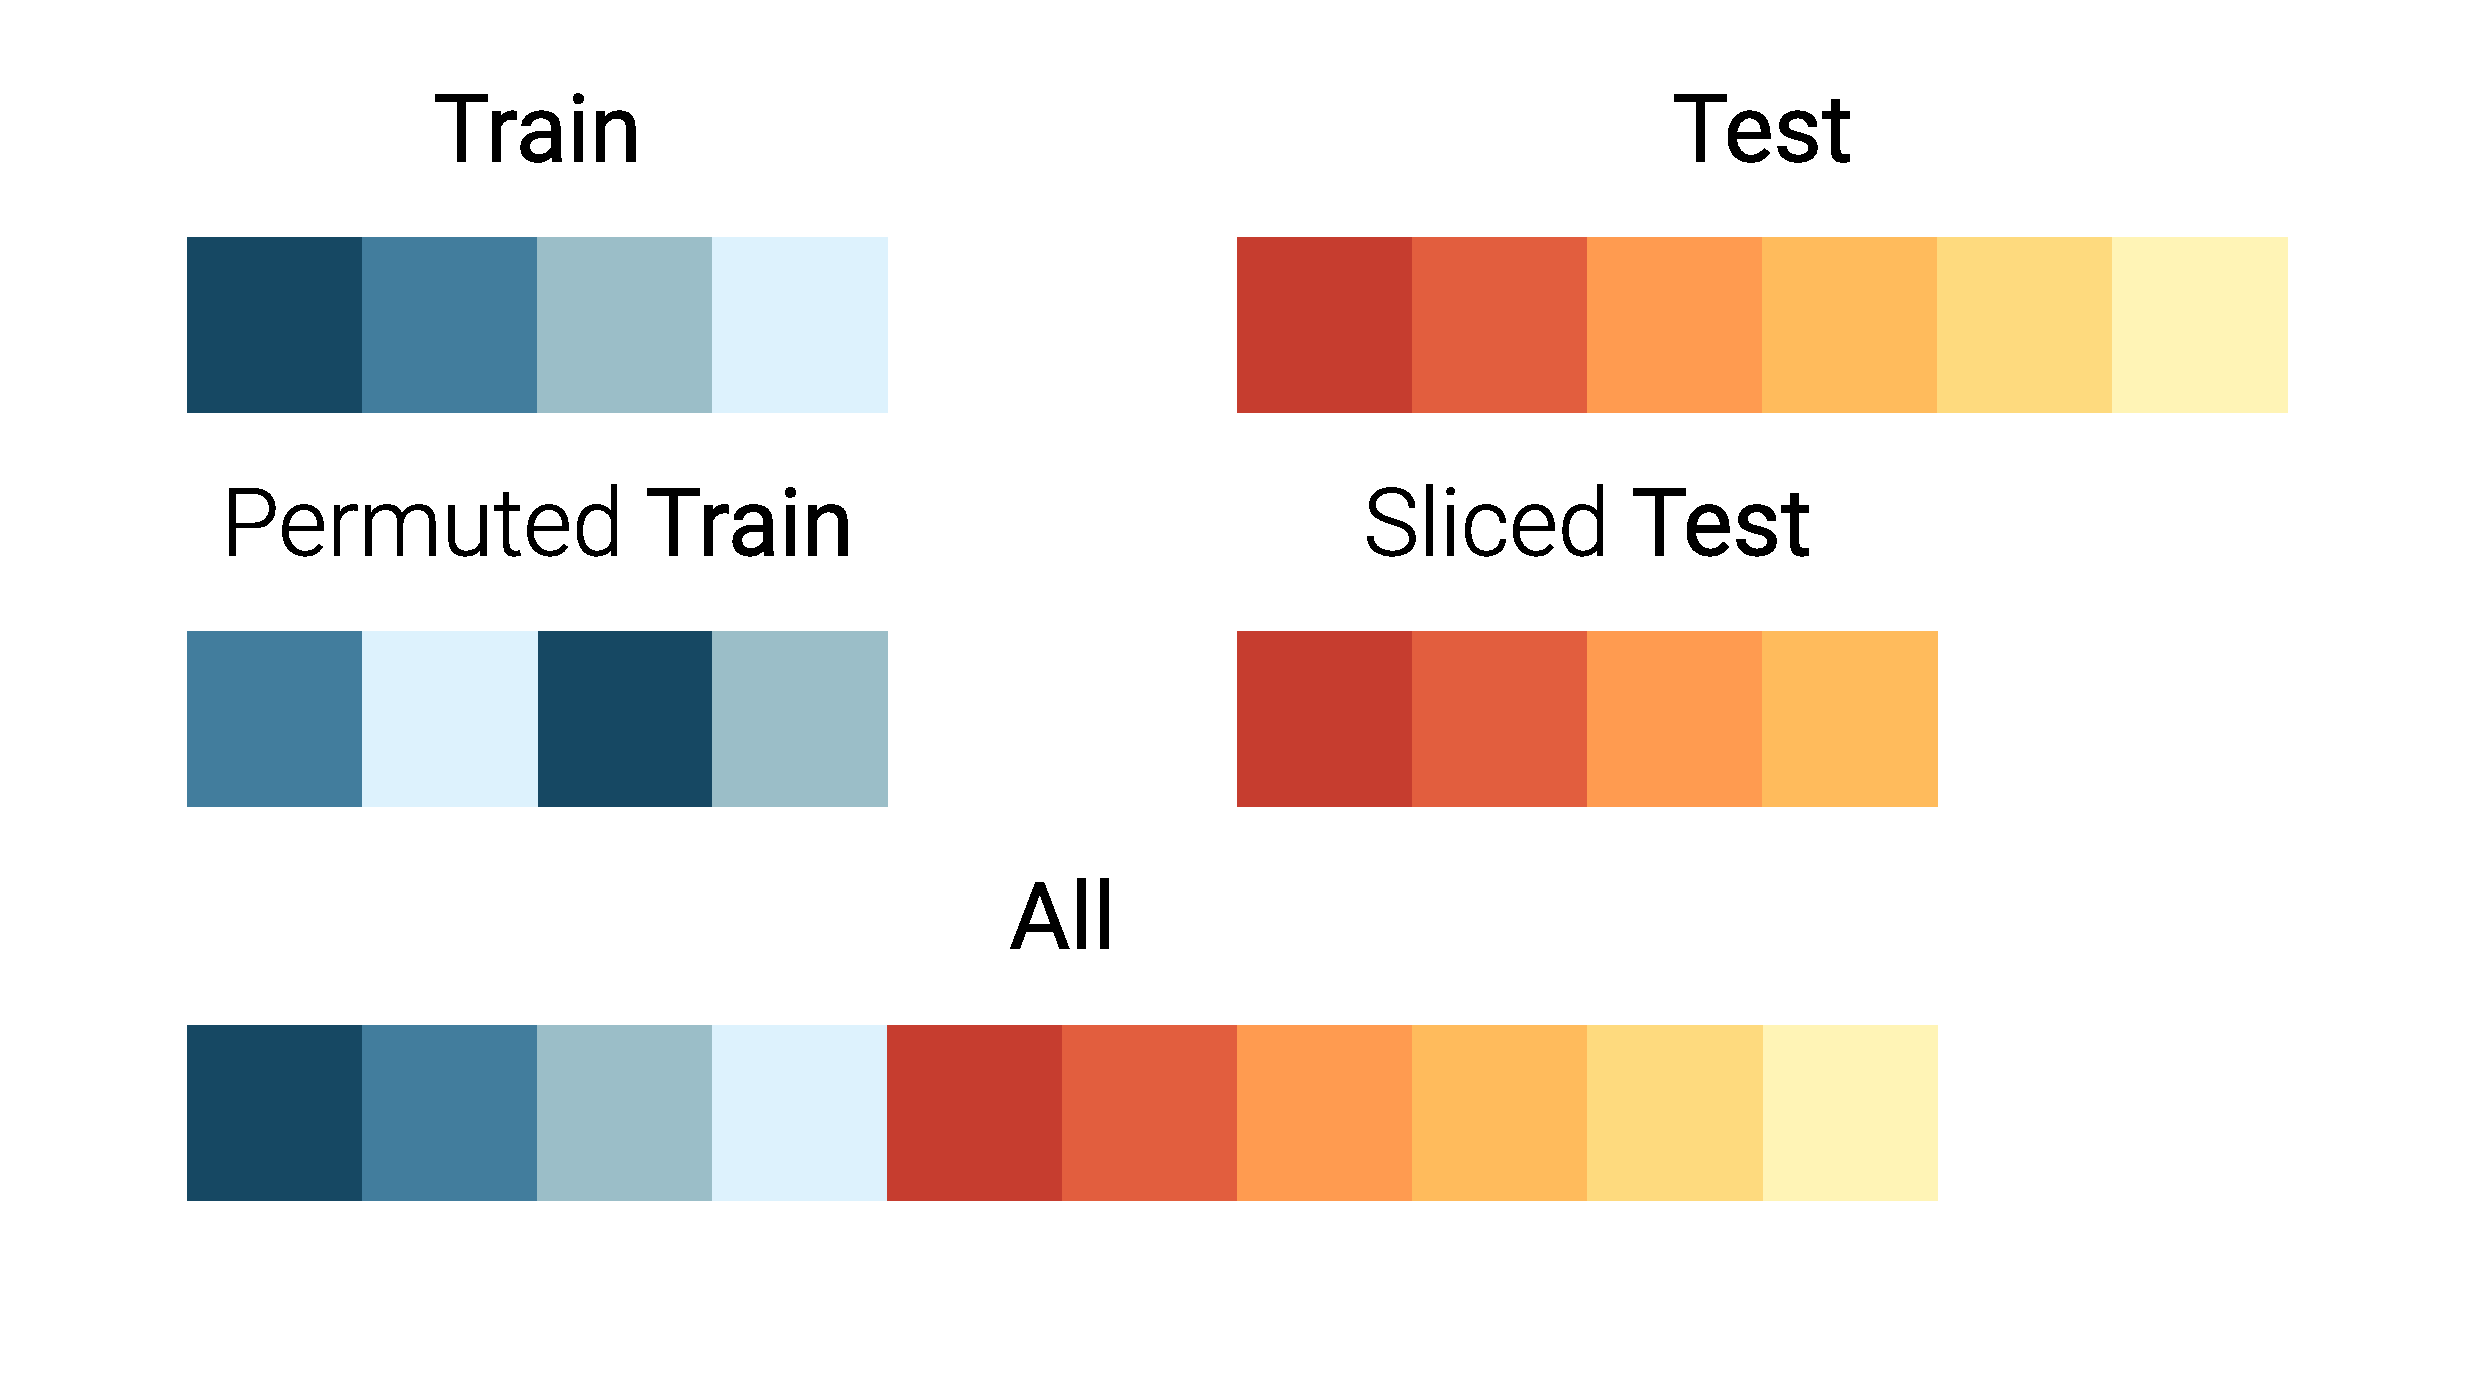
\includegraphics[width=\columnwidth]{visualizations/action_sets_vis_new.pdf}
    % 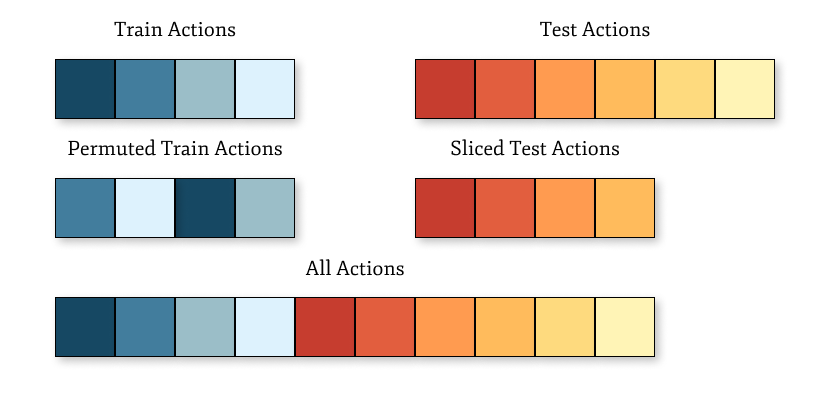
\includegraphics[width=\columnwidth]{visualizations/action_sets_vis_2.png}
    \caption{\textbf{Variable Action Spaces:} We consider four types of novel action spaces different from the one used during training. \emph{Permuted Train Actions} maintains the action set contents but reorders its elements. \emph{Test Actions} introduces a completely new action set with an increased size. It is important to consider that some models may be architecturally limited to a fixed action set size. To evaluate the performance of such models on unseen actions, we adjust the size of a new set to be compatible with the model output. Therefore, we slice the first actions from the \emph{Test Actions} set. Lastly, a new action space might include both the seen \emph{Train} and unseen \emph{Test} actions, depicted as the \emph{All Actions} set.}
    \label{fig:action_sets_viz}
    \vskip -0.2in
\end{figure}

\begin{figure*}[t]
    \vskip 0.2in
    \centering
    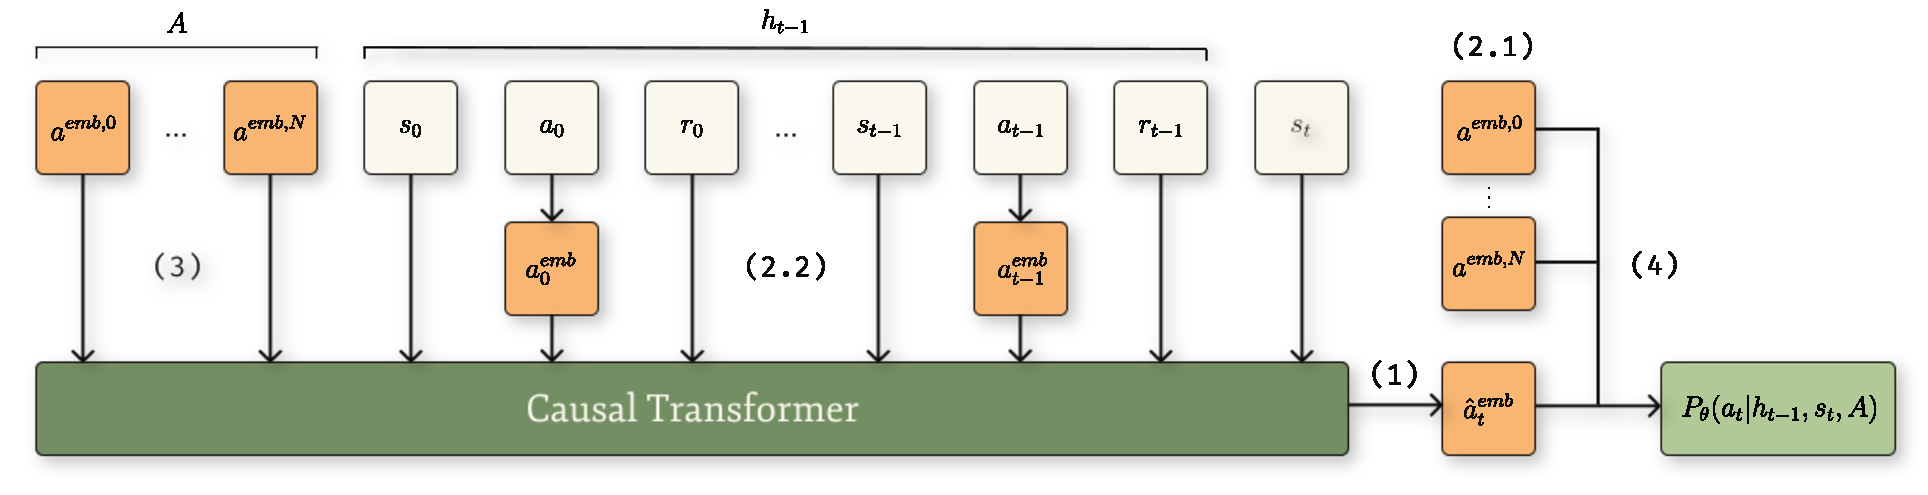
\includegraphics[width=\textwidth]{visualizations/model_vis.pdf}
    \caption{\textbf{Headless-AD Architecture:} Compared to AD, Headless-AD introduces four new components. (1) We remove the output linear head, making the model directly predict the action embedding. That allows us to avoid a direct connection between the model and action space size, contents and ordering. (2.1) At each training step, we generate random action embeddings for each action in the action set. (2.2) We convert actions in the context into their embeddings and pass them as the model input. This prepares the model for unseen actions, forcing it to infer action semantics from the context. (3) As the model loses prior knowledge about action space structure, we pass the generated action embeddings as a prompt to aid the model in sensible action selection. (4) We convert a prediction vector into a distribution over actions based on the similarities between the prediction and previously generated action embeddings. To increase the probability of correct actions, we use contrastive loss instead of cross-entropy.}
    \label{fig:model_vis}
    \vskip -0.2in
\end{figure*}


The transformer architecture, first introduced by \citet{vaswani2017attention}, has been widely adopted in key areas of machine learning, including natural language processing \citep{radford2018improving, devlin2018bert}, computer vision \citep{dosovitskiy2020image} and sequential decision-making \citep{chen2021decision}. One major feature of transformers is in-context learning (ICL), which makes it possible for them to adapt to new tasks after extensive pre-training \citep{brown2020language, liu2023pre}. Recent developments, such as Algorithm Distillation (AD) by \citet{laskin2022context} and Decision Pretrained Transformer (DPT) by \citet{lee2023supervised}, have successfully employed transformer ICL abilities in sequential decision-making. These models are capable of predicting the next action based on a query state and history of environment interactions, which inform them about task objectives and environment dynamics. While effective at generalizing across various reward distributions \citep{laskin2022context, lee2023supervised} and transition functions \citep{raparthy2023generalization}, their adaptability to new action spaces remains unexplored and limited by architectural constraints.

Creating models that can adapt to new action spaces is essential for building the foundation of decision-making systems in order to enable large-scale pretraining across various environments and address real-world problems \citep{jain2020generalization, chandak2020lifelong, london2020offline, jain2021know}. With this in mind, our research focuses on variable discrete action spaces, with the notion of variability illustrated in the \Cref{fig:action_sets_viz}. In our study, we reveal the limitations of the Algorithm Distillation model from prior work, such as its diminished performance upon changes in action semantics as well as architectural constraints when handling varying action space sizes (see \Cref{fig:bad_ad}). 
% The reason for these limitations is the classifier-like structure of AD and the fixed output dimension of the output layer.


Our solution, \textbf{Headless-AD}, is an architecture and training methodology tailored to effective generalization on new action spaces. We employ an approach similar to Wolterpinger \citep{dulac2015deep} and Headless-LLM \citep{godey2023headless} by encoding actions with random embeddings \citep{kirsch2023towards} and directly predicting these embeddings. This way, we remove the direct connection between the model output layer and the action space structure. 

Through experiments using Bernoulli and contextual bandits, and a darkroom environment with changing action spaces, we demonstrate that Headless-AD is capable of matching the performance of the original data generation algorithm and scaling to action spaces up to $\textbf{5x}$ larger than those seen during training. We also observed that Headless-AD can even outperform AD when they are both trained for the same action space, especially when evaluated on larger action sets. To summarize, our contributions are as follows:
\begin{itemize}
    \item We show that AD struggles with generalization on novel action spaces (\Cref{section:ad_struggles}).
    \item We extend AD with a modified model architecture and a training strategy, called \textbf{Headless-AD}, for it to acquire the ability to adapt to new discrete action spaces (\Cref{section:headless_ad}). We demonstrate the strong generalization capabilities of Headless-AD on Bernoulli and contextual bandits, and darkroom environments (\Cref{section:experiments}).
    \item We perform ablations on the loss and the prompt format to highlight the importance of Headless-AD's design choices (\Cref{section:ablations}).
\end{itemize}
% Remove it and see that the specing between the items above becomes too large
% This is a quick-fix
\vphantom{loh}\\

